\chapter{Results Appendix}
\label{app:R}

\begin{figure}[h]
    \centering
    \begin{subfigure}{0.3\textwidth}
        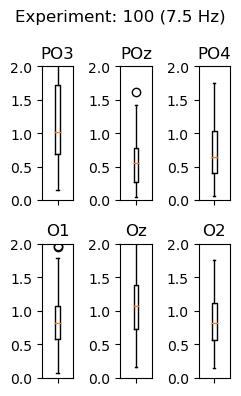
\includegraphics[width=\linewidth]{images/appendix/10075.png}
        \label{fig:10075}
    \end{subfigure}
    \hfill
    \begin{subfigure}{0.3\textwidth}
        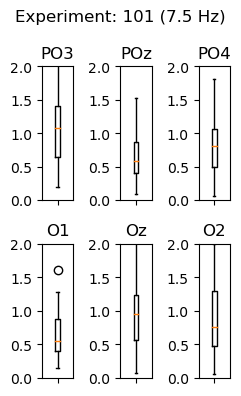
\includegraphics[width=\linewidth]{images/appendix/10175.png}
        \label{fig:10175}
    \end{subfigure}
    \hfill
    \begin{subfigure}{0.3\textwidth}
        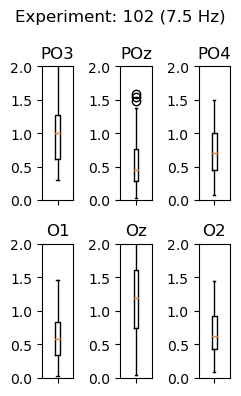
\includegraphics[width=\linewidth]{images/appendix/10275.png}
        \label{fig:10275}
    \end{subfigure}
    \caption{Experiment 1 - Conditions 0, 1, and 2: Boxplots per hemisphere.}
    \label{fig:1-675}
\end{figure}


\begin{figure}[ht]
    \centering
    \begin{subfigure}{0.25\linewidth}
        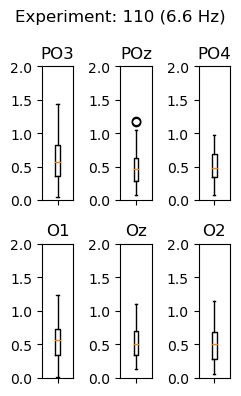
\includegraphics[width=\linewidth]{images/appendix/11066.png}
        \label{fig:11066}
    \end{subfigure}
    \begin{subfigure}{0.25\linewidth}
        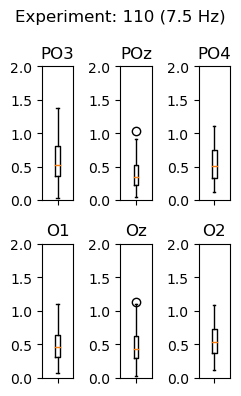
\includegraphics[width=\linewidth]{images/appendix/11075.png}
        \label{fig:11075}
    \end{subfigure}
    
    \begin{subfigure}{0.25\linewidth}
        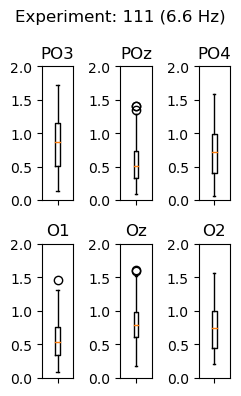
\includegraphics[width=\linewidth]{images/appendix/11166.png}
        \label{fig:11166}
    \end{subfigure}
    \begin{subfigure}{0.25\linewidth}
        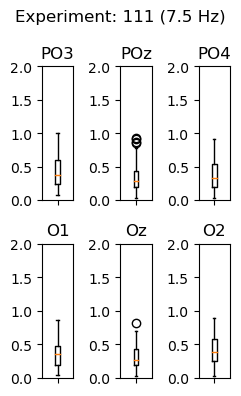
\includegraphics[width=\linewidth]{images/appendix/11175.png}
        \label{fig:11175}
    \end{subfigure}
        
    \begin{subfigure}{0.25\linewidth}
        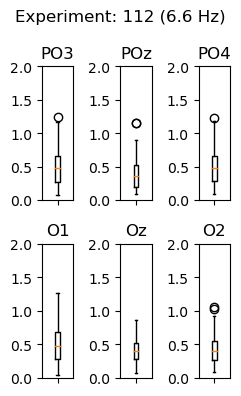
\includegraphics[width=\linewidth]{images/appendix/11266.png}
        \label{fig:11266}
    \end{subfigure}
    \begin{subfigure}{0.25\linewidth}
        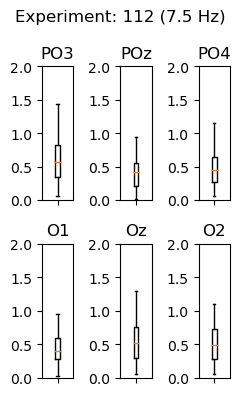
\includegraphics[width=\linewidth]{images/appendix/11275.png}
        \label{fig:11275}
    \end{subfigure}
    \caption{Experiment 2 - Conditions 0, 1, and 2: Boxplots per hemisphere.}
    \label{fig:2-6675}
\end{figure}

\begin{figure}[ht]
    \centering
    \begin{subfigure}{0.3\textwidth}
        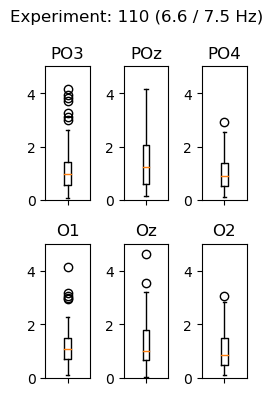
\includegraphics[width=\linewidth]{images/results/1106675.png}
        \label{fig:1106675}
    \end{subfigure}
    \hfill
    \begin{subfigure}{0.3\textwidth}
        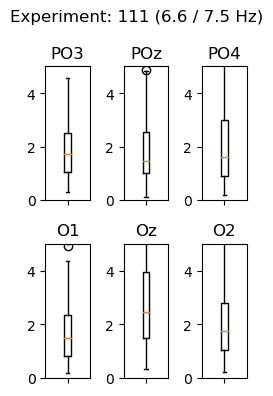
\includegraphics[width=\linewidth]{images/results/1116675.png}
        \label{fig:1116675}
    \end{subfigure}
    \hfill
    \begin{subfigure}{0.3\textwidth}
        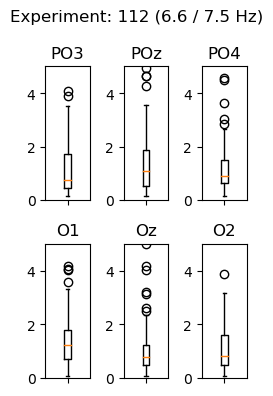
\includegraphics[width=\linewidth]{images/results/1126675.png}
        \label{fig:1126675}
    \end{subfigure}
    \caption{Experiment 2: Boxplot comparisons of amplitude ratios for the different conditions.}
    \label{fig:2-66/75}
\end{figure}


\begin{figure}[ht]
    \centering
    \begin{subfigure}{0.25\linewidth}
        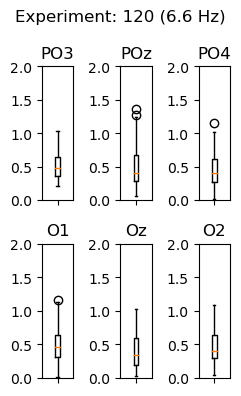
\includegraphics[width=\linewidth]{images/appendix/12066.png}
        \label{fig:12066}
    \end{subfigure}
    \begin{subfigure}{0.25\linewidth}
        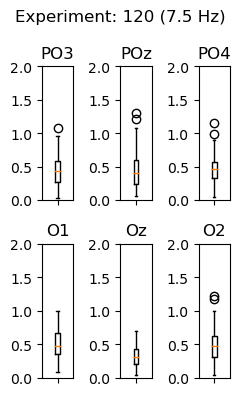
\includegraphics[width=\linewidth]{images/appendix/12075.png}
        \label{fig:12075}
    \end{subfigure}
    \caption{Experiment 3 - Boxplots per hemisphere.}
    \label{fig:3-6675}
\end{figure}


\begin{figure}[ht]
    \centering
    \begin{subfigure}{0.25\linewidth}
        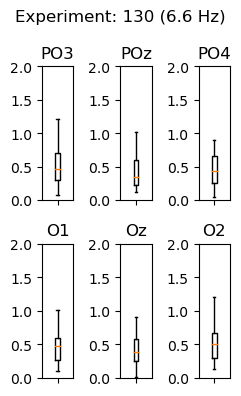
\includegraphics[width=\linewidth]{images/appendix/13066.png}
        \label{fig:13066}
    \end{subfigure}
    \begin{subfigure}{0.25\linewidth}
        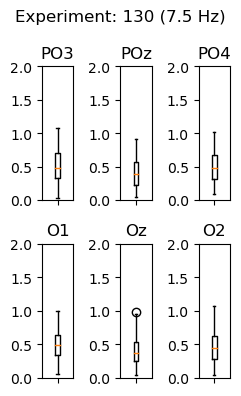
\includegraphics[width=\linewidth]{images/appendix/13075.png}
        \label{fig:13075}
    \end{subfigure}
    
    \begin{subfigure}{0.25\linewidth}
        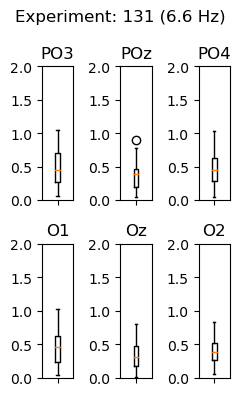
\includegraphics[width=\linewidth]{images/appendix/13166.png}
        \label{fig:13166}
    \end{subfigure}
    \begin{subfigure}{0.25\linewidth}
        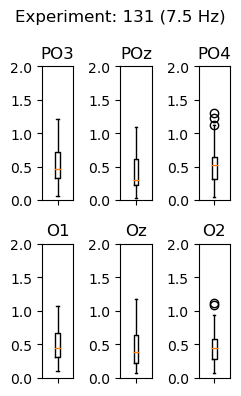
\includegraphics[width=\linewidth]{images/appendix/13175.png}
        \label{fig:13175}
    \end{subfigure}
    \caption{Experiment 4 - Conditions 0, 1, and 2: Boxplots per hemisphere.}
    \label{fig:4-6675}
\end{figure}


\begin{figure}[ht]
    \centering
    \begin{subfigure}{0.25\textwidth}
        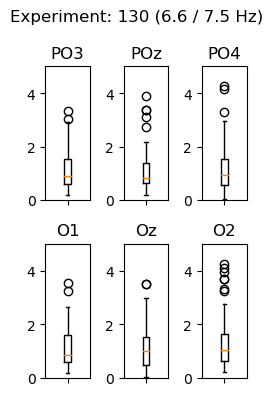
\includegraphics[width=\linewidth]{images/results/1306675.png}
        \label{fig:1306675}
    \end{subfigure}
    \begin{subfigure}{0.25\textwidth}
        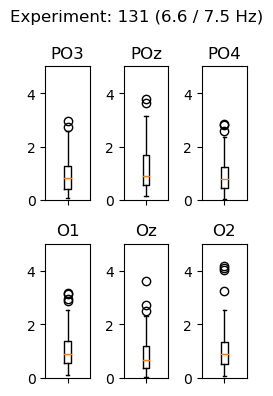
\includegraphics[width=\linewidth]{images/results/1316675.png}
        \label{fig:1316675}
    \end{subfigure}
    \caption{Experiment 4 - Conditions 0 and 1: Boxplots per hemisphere.}
    \label{fig:4-66/75}
\end{figure}
